\documentclass[ignorenonframetext,]{beamer}
\setbeamertemplate{caption}[numbered]
\setbeamertemplate{caption label separator}{: }
\setbeamercolor{caption name}{fg=normal text.fg}
\beamertemplatenavigationsymbolsempty
\usepackage{lmodern}
\usepackage{pgfplots}
\usepackage{amssymb,amsmath}
\usepackage{ifxetex,ifluatex}
\usepackage{fixltx2e} % provides \textsubscript
\ifnum 0\ifxetex 1\fi\ifluatex 1\fi=0 % if pdftex
  \usepackage[T1]{fontenc}
  \usepackage[utf8]{inputenc}
\else % if luatex or xelatex
  \ifxetex
    \usepackage{mathspec}
  \else
    \usepackage{fontspec}
  \fi
  \defaultfontfeatures{Ligatures=TeX,Scale=MatchLowercase}
\fi
% use upquote if available, for straight quotes in verbatim environments
\IfFileExists{upquote.sty}{\usepackage{upquote}}{}
% use microtype if available
\IfFileExists{microtype.sty}{%
\usepackage{microtype}
\UseMicrotypeSet[protrusion]{basicmath} % disable protrusion for tt fonts
}{}
\newif\ifbibliography
\hypersetup{
            pdfborder={0 0 0},
            breaklinks=true}
\usepackage{graphicx,grffile}
\makeatletter
\def\maxwidth{\ifdim\Gin@nat@width>\linewidth\linewidth\else\Gin@nat@width\fi}
\def\maxheight{\ifdim\Gin@nat@height>\textheight0.8\textheight\else\Gin@nat@height\fi}
\makeatother
% Scale images if necessary, so that they will not overflow the page
% margins by default, and it is still possible to overwrite the defaults
% using explicit options in \includegraphics[width, height, ...]{}
\setkeys{Gin}{width=\maxwidth,height=\maxheight,keepaspectratio}

% Prevent slide breaks in the middle of a paragraph:
\widowpenalties 1 10000
\raggedbottom

\AtBeginPart{
  \let\insertpartnumber\relax
  \let\partname\relax
  \frame{\partpage}
}
\AtBeginSection{
  \ifbibliography
  \else
    \let\insertsectionnumber\relax
    \let\sectionname\relax
    \frame{\sectionpage}
  \fi
}
\AtBeginSubsection{
  \let\insertsubsectionnumber\relax
  \let\subsectionname\relax
  \frame{\subsectionpage}
}

\setlength{\parindent}{0pt}
\setlength{\parskip}{6pt plus 2pt minus 1pt}
\setlength{\emergencystretch}{3em}  % prevent overfull lines
\providecommand{\tightlist}{%
  \setlength{\itemsep}{0pt}\setlength{\parskip}{0pt}}
\setcounter{secnumdepth}{0}

\date{}

\begin{document}

\begin{frame}{Chapter 5 - Logarithmic Functions}

\begin{itemize}
\tightlist
\item
  \protect\hyperlink{5.1-logarithms-and-their-properties}{5.1 Logarithms
  and their Properties}
\item
  \protect\hyperlink{5.2-logarithms-and-exponential-models}{5.2
  Logarithms and Exponential Models}
\item
  \protect\hyperlink{5.3-the-logarithmic-function}{5.3 The Logarithmic
  Function}
\item
  \protect\hyperlink{5.4-logarithmic-scales}{5.4 Logarithmic Scales}
\item
  \protect\hyperlink{chapter-5-review}{Chapter 5 Review}
\end{itemize}

\end{frame}

\begin{frame}{5.1 Logarithms and their Properties}

\begin{block}{Objectives}

\begin{itemize}
\tightlist
\item
  I can convert between exponential and logarithmic statements.
\item
  I can apply the properties of logarithms to solve equations.
\end{itemize}

\end{block}

\end{frame}

\begin{frame}{Common Logarithm Function}

\begin{itemize}
\tightlist
\item
  If \(x\) is a positive number, \(\log(x)\) is the exponent of 10 that
  gives \(x\).
\item
  In other words, if \(y = \log(x)\) then \(10^y = x\).
\end{itemize}

\end{frame}

\begin{frame}{Example 1}

Rewrite the following statements using exponents instead of logs.

\begin{itemize}
\tightlist
\item
  \(\log(4) = 0.602\)
\item
  \(\log(q) = z\)
\end{itemize}

\end{frame}

\begin{frame}{Example 2}

Evaluate with a calculator.

\begin{itemize}
\tightlist
\item
  \(\log(10^7)\)
\item
  \(10^{\log(5)}\)
\end{itemize}

\end{frame}

\begin{frame}{Properties of the Common Logarithm}

\begin{itemize}
\tightlist
\item
  By definition, \(y = \log(x)\) means \(10^y = x\). In particular,
  \(\log(1) = 0\) and \(\log(10) = 1\).
\item
  The functions \(10^x\) and \(\log(x)\) are inverses, so they ``undo''
  each other: \(\log(10^x) = x\) for all \(x\) and \(10^{\log(x)} = x\)
  for \(x > 0\).
\item
  For \(a\) and \(b\) both positive and any value of \(t\):
  \(\log(ab) = \log(a) + \log(b)\),
  \(\log\left(\frac{a}{b}\right) = \log(a) - \log(b)\), and
  \(\log(b^t) = t\log(b)\).
\end{itemize}

\end{frame}

\begin{frame}{Example 3}

Solve the equation using logs. \[(1.45)^x = 25\]

\end{frame}

\begin{frame}{The Natural Logarithm}

\begin{itemize}
\tightlist
\item
  For \(x > 0\), \(\ln(x)\) is the power of \(e\) that gives \(x\).
\item
  In symbols, \(\ln(x) = y\) means \(e^y = x\), and \(y\) is called the
  \textbf{natural logarithm} of \(x\).
\end{itemize}

\end{frame}

\begin{frame}{Properties of the Natural Logarithm}

\begin{itemize}
\tightlist
\item
  By definition, \(y = \ln(x)\) means \(x = e^y\). In particular,
  \(\ln 1 = 0\) and \(\ln e = 1\).
\item
  The functions \(e^x\) and \(\ln x\) are inverses, so they ``undo''
  each other: \(\ln(e^x) = x\) for all \(x\) and \(e^{\ln x} = x\) for
  \(x > 0\).
\item
  For \(a\) and \(b\) both positive and any value of \(t\):
  \(\ln (ab) = \ln a + \ln b\),
  \(\ln \left(\frac{a}{b}\right) = \ln a - \ln b\), and
  \(\ln (b^t) = t\ln b\).
\end{itemize}

\end{frame}

\begin{frame}{Example 4}

Solve the equation using logs. \[10 = 22(0.87)^q\]

\end{frame}

\begin{frame}{Assignments}

\begin{itemize}
\tightlist
\item
  Day 1 Page 185, 1-17 odd
\item
  Day 2 Page 186, 19-33 odd
\item
  Day 3 Page 187, 35-51 odd (not 45, 51)
\end{itemize}

\end{frame}

\begin{frame}{5.1 Day 2}

\begin{block}{Agenda}

\begin{itemize}
\tightlist
\item
  Warm-Up Problem
\item
  Day 1 Page 185, 1-17 odd Assignment Questions
\item
  Misconceptions Involving Logs Notes
\item
  Work time
\end{itemize}

\end{block}

\begin{block}{Objectives}

\begin{itemize}
\tightlist
\item
  I can convert between exponential and logarithmic statements.
\item
  I can apply the properties of logarithms to solve equations.
\end{itemize}

\end{block}

\end{frame}

\begin{frame}{Warm-Up Problem}

Simplify. \[log(\sqrt{10000})\]

Solve the equation using logs. \[\frac{2}{7} = (0.6)^{2t}\]

\emph{Properties of the Natural Logarithm}

\begin{itemize}
\tightlist
\item
  The functions \(e^x\) and \(\ln x\) are inverses, so they ``undo''
  each other: \(\ln(e^x) = x\) for all \(x\) and \(e^{\ln x} = x\) for
  \(x > 0\).
\item
  For \(a\) and \(b\) both positive and any value of \(t\):
  \(\ln (ab) = \ln a + \ln b\),
  \(\ln \left(\frac{a}{b}\right) = \ln a - \ln b\), and
  \(\ln (b^t) = t\ln b\).
\end{itemize}

\end{frame}

\begin{frame}{Questions on Page 185, 1-17 odd?}

\end{frame}

\begin{frame}{Misconceptions Involving Logs Notes}

\begin{itemize}
\tightlist
\item
  \(\log(a+b) \neq \log(a) + \log(b)\)
\item
  \(\log(a-b) \neq \log(a) - \log(b)\)
\item
  \(\log(ab) \neq (\log(a))(\log(b))\)
\item
  \(\log\left(\frac{a}{b}\right) \neq \frac{\log(a)}{\log(b)}\)
\item
  \(\log\left(\frac{1}{a}\right) \neq \frac{1}{\log(a)}\)
\end{itemize}

\end{frame}

\begin{frame}{Work time on Assignments}

\begin{itemize}
\tightlist
\item
  Day 1 Page 185, 1-17 odd
\item
  Day 2 Page 186, 19-33 odd
\item
  Day 3 Page 187, 35-51 odd (not 45, 51)
\item
  All Due Wednesday
\end{itemize}

\end{frame}

\begin{frame}{5.1 Day 3}

\begin{block}{Agenda}

\begin{itemize}
\tightlist
\item
  Warm-Up Problem
\item
  Page 186, 19-33 odd Assignment Questions
\item
  Work time
\end{itemize}

\end{block}

\begin{block}{Objectives}

\begin{itemize}
\tightlist
\item
  I can convert between exponential and logarithmic statements.
\item
  I can apply the properties of logarithms to solve equations.
\end{itemize}

\end{block}

\end{frame}

\begin{frame}{Warm-Up Problem}

\begin{enumerate}
\def\labelenumi{\arabic{enumi}.}
\item
  Use the properties of logarithms to solve for \(x\).
  \[\log(3(2)^x) = 8\]
\item
  Solve the equation exactly for \(x\). \[e^{x+5} = 7(2)^x\]
\end{enumerate}

\emph{Properties of the Natural Logarithm}

\begin{itemize}
\tightlist
\item
  The functions \(e^x\) and \(\ln x\) are inverses, so they ``undo''
  each other: \(\ln(e^x) = x\) for all \(x\) and \(e^{\ln x} = x\) for
  \(x > 0\).
\item
  For \(a\) and \(b\) both positive and any value of \(t\):
  \(\ln (ab) = \ln a + \ln b\),
  \(\ln \left(\frac{a}{b}\right) = \ln a - \ln b\), and
  \(\ln (b^t) = t\ln b\).
\end{itemize}

\end{frame}

\begin{frame}{Warm-Up Problem 1 Solution}

\begin{enumerate}
\def\labelenumi{\arabic{enumi}.}
\tightlist
\item
  Use the properties of logarithms to solve for \(x\).
\end{enumerate}

\begin{align*}
\log(3(2)^x) &= 8 \\
\log(3)+\log(2^x) &= 8 \\
\log(3)+x\log(2) &= 8 \\
x\log(2) &= 8-\log(3) \\
x &= \frac{8-\log(3)}{\log(2)} \\
\end{align*}

\end{frame}

\begin{frame}{Warm-Up Problem 2 Solution}

\begin{enumerate}
\def\labelenumi{\arabic{enumi}.}
\setcounter{enumi}{1}
\tightlist
\item
  Solve the equation exactly for \(x\).
\end{enumerate}

\begin{align*}
e^{x+5} &= 7(2)^x \\
\ln(e^{x+5}) &= \ln(7(2)^x) \\
x+5 &= \ln(7)+\ln((2)^x) \\
x+5 &= \ln(7)+x\ln(2) \\
x-x\ln(2) &= \ln(7)-5 \\
x(1-\ln(2)) &= \ln(7)-5 \\
x &= \frac{\ln(7)-5}{1-\ln(2)}
\end{align*}

\end{frame}

\begin{frame}{Questions on Page 186, 19-33 odd?}

\end{frame}

\begin{frame}{Work time on Assignments}

\begin{itemize}
\tightlist
\item
  Day 1 Page 185, 1-17 odd
\item
  Day 2 Page 186, 19-33 odd
\item
  Day 3 Page 187, 35-51 odd (not 45, 51)
\item
  All Due Tomorrow
\end{itemize}

\end{frame}

\begin{frame}{5.2 Logarithms and Exponential Models}

\begin{block}{Objectives}

\begin{itemize}
\tightlist
\item
  I can use logarithms to solve exponential equations.
\item
  I can setup an exponential equation to model doubling and half-life.
\end{itemize}

\end{block}

\end{frame}

\begin{frame}{Example 1 - Doubling Time}

You place 1000 MMK in a KBZ Bank fixed deposit bank account. According
to their website, a 1 month term account earns 9\% interest, 3 months
earns 9.25\%, 6 months earns 9.5\%, 9 months earns 9.75\%, and 12 months
earns 10\%.

\begin{itemize}
\tightlist
\item
  How often is a fixed account compounded at KBZ Bank?
\item
  \(\$ 1 \approx 1300\) MMK. If you deposit \$1000000 into the KBZ fixed
  deposit account with a 12 month term, how much interest would you
  earn?
\item
  If you open an account with 1000 MMK, how long would it take to double
  your money with each term account?
\end{itemize}

\end{frame}

\begin{frame}{Example 1 - Doubling Time - Solution}

You place 1000 MMK in a KBZ Bank fixed deposit bank account. According
to their website, a 1 month term account earns 9\% interest, 3 months
earns 9.25\%, 6 months earns 9.5\%, 9 months earns 9.75\%, and 12 months
earns 10\%.

\begin{itemize}
\tightlist
\item
  How often is a fixed account compounded at KBZ Bank? Depends on the
  term. \(B = P\left(1+\frac{r}{n}\right)^{nt}\)
\item
  \(\$ 1 \approx 1300\) MMK. If you deposit \$1,000,000 into the KBZ
  fixed deposit account with a 12 month term, how much interest would
  you earn? \(P = 1000000\), \(t = 1\), \(r = 0.1\), \(n = 1\), so
  \(B = 1000000\left(1+\frac{0.1}{1}\right)^{1(1)} = 1100000\). This
  means they earn \$100000 in interest.
\item
  If you open an account with 1000 MMK, how long would it take to double
  your money with each term account?
\item
  1 month: \(n = 12\) and \(r = 0.09\), so
  \(2000 = 1000\left(1+\frac{0.09}{12}\right)^{12t}\).
  \(t = \ln(2)/(12\ln\left(1+\frac{0.09}{12}\right)) \approx 7.730\)
  years.
\item
  3 months: \(n = 4\) and \(r = 0.0925\), so
  \(2000 = 1000\left(1+\frac{0.0925}{4}\right)^{4t}\).
  \(t = \ln(2)/(4\ln\left(1+\frac{0.0925}{4}\right)) \approx 7.579\)
  years.
\item
  6 months: \(n = 2\) and \(r = 0.095\), so
  \(2000 = 1000\left(1+\frac{0.095}{2}\right)^{2t}\).
  \(t = \ln(2)/(2\ln\left(1+\frac{0.095}{2}\right)) \approx 7.468\)
  years.
\item
  9 months: \(n = 12/9\) and \(r = 0.0975\), so
  \(2000 = 1000\left(1+\frac{0.0975}{12/9}\right)^{(12/9)t}\).
  \(t = \ln(2)/((12/9)\ln\left(1+\frac{0.0975}{(12/9)}\right)) \approx 7.366\)
  years.
\item
  12 months: \(n = 1\) and \(r = 0.1\), so
  \(2000 = 1000\left(1+\frac{0.1}{1}\right)^{(1)t}\).
  \(t = \ln(2)/(1\ln\left(1+\frac{0.1}{1}\right)) \approx 7.272\) years.
\end{itemize}

\end{frame}

\begin{frame}{Example 2 - Half-Life}

The Chernobyl expolosion in 1986 initially had a radiation reading of
300 Sv/hr near the reactor core. After 22 years, the radiation levels
inside the reactor hall were about 34 Sv/hr. More than half of people
exponsed to 5 Sv will die from the radiation.

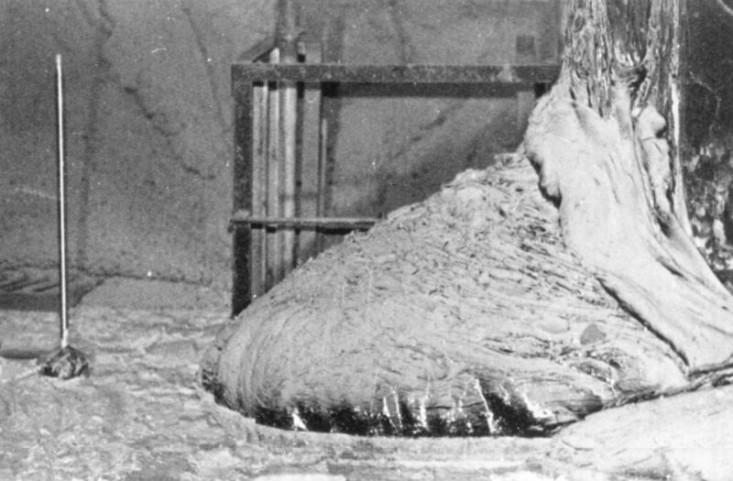
\includegraphics{media/reactor.jpg}

\begin{itemize}
\tightlist
\item
  What is the rate at which the radiation is decaying? Assume
  exponential decay.
\item
  How long was it until half the radiation remained?
\item
  How long would it take to receive a lethal dose of radiation in the
  reactor hall today?
\end{itemize}

\end{frame}

\begin{frame}{Example 2 - Half-Life - Solution}

The Chernobyl expolosion in 1986 initially had a radiation reading of
300 Sv/hr near the reactor core. After 22 years, the radiation levels
inside the reactor hall were about 34 Sv/hr. More than half of people
exponsed to 5 Sv will die from the radiation.

\begin{itemize}
\tightlist
\item
  What is the rate at which the radiation is decaying? Assume
  exponential decay. \(34 = 300e^{k(22)}\), so
  \(k = \ln(34/300)/22 \approx -0.098973725\), so down by 9.897\%.
\item
  How long was it until half the radiation remained?
  \(150 = 300e^{-0.098973725t}\), so
  \(t = \ln(150/300)/(-0.098973725) \approx 7.003345388\) years.
\item
  How long would it take to receive a lethal dose of radiation in the
  reactor hall today?
  \(Sv = 300e^{-0.098973725(30)} \approx 15.40312983\), so 15 Sv/hr
  would mean 5 Sv in 20 minutes.
\end{itemize}

\end{frame}

\begin{frame}{Converting Between \(Q = ab^t\) and \(Q = ae^{kt}\)}

Any exponential function can be written in either of the two forms:
\[Q = ab^t \text{ or } Q = ae^{kt}\] If \(b = e^k\), so \(k = \ln(b)\),
the two formulas represent the same function.

\end{frame}

\begin{frame}{Example 3}

Convert to the form \(Q = ab^t\). \[Q = 0.3e^{0.7t}\]

\end{frame}

\begin{frame}{Example 3 - Solution}

Convert to the form \(Q = ab^t\).
\[Q = 0.3e^{0.7t} = 0.3(e^{0.7})^t \approx 0.3(2.01375)^t\]

\end{frame}

\begin{frame}{Example 4}

Convert to the form \(Q = ae^{kt}\). Give the starting value \(a\), the
growth rate \(r\), and the continuous growth rate \(k\).
\[Q = 5(2)^{t/8}\]

\end{frame}

\begin{frame}{Example 4}

Convert to the form \(Q = ae^{kt}\). Give the starting value \(a\), the
growth rate \(r\), and the continuous growth rate \(k\).

\(Q = 5(2)^{t/8} = 5\left(2^{\frac{1}{8}}\right)^t\), so
\(e^k = 2^{\frac{1}{8}}\) and then
\(k = \ln\left(2^{\frac{1}{8}}\right) \approx 0.08664\). Thus,
\(Q = 5e^{0.08664t}\).

\end{frame}

\begin{frame}{5.2 Assignments and 5.1 Homework Check}

\begin{itemize}
\tightlist
\item
  Homework Check: 5.1, Page 185, 1-51 odd (not 45, 51)
\item
  Day 1, Page 194, 1-19 odd
\item
  Day 2, Page 194, 21-51 odd (not 43)
\item
  5.2 Assignments are due Monday
\end{itemize}

\end{frame}

\begin{frame}{5.2 Assignment Questions?}

\begin{itemize}
\tightlist
\item
  Day 1, Page 194, 1-19 odd
\item
  Day 2, Page 194, 21-51 odd (not 43)
\item
  5.2 Assignments are due Monday
\end{itemize}

\end{frame}

\begin{frame}{5.3 The Logarithmic Function}

\begin{block}{Agenda}

\begin{itemize}
\tightlist
\item
  Homework Check: 5.2 Page 194, 1-51 odd (not 43)
\item
  5.3 Notes
\item
  Work time
\end{itemize}

\end{block}

\begin{block}{Objectives}

\begin{itemize}
\tightlist
\item
  I can graph \(\log(x)\) and \(\ln(x)\) using their inverse functions.
\item
  I can solve word problems involving chemical acidity, decibals, and
  orders of magnitude.
\end{itemize}

\end{block}

\end{frame}

\begin{frame}{The Graph, Domain, and Range of the Common Logarithm}

\(\log(x)\) is the inverse of \(10^x\), so the graph of \(\log(x)\) is
the reflection across \(y = x\) of \(10^x\).

\begin{tikzpicture}
\begin{axis}[xlabel={$x$},ylabel={$y$},axis lines=middle,xmin=-2,xmax=11,ymin=-2,ymax=11]
\addplot[blue,no marks,samples=200,domain=-1:10] {log10(x)} node[above,pos=1] {$y = \log(x)$};
\addplot[red,no marks,samples=200,domain=-1:1] {10^x} node[above,pos=1] {$y = 10^x$};
\addplot[dashed,domain=-1:10] {x} node[above,pos=1] {$y = x$};
\end{axis}
\end{tikzpicture}

The domain of \(y = 10^x\) is all real numbers and the range is all
positive real numbers. The domain of \(y = \log(x)\) is all positive
real numbers and the range is all real numbers.

\end{frame}

\begin{frame}{Graph of Natural Logarithm}

The graph of \(y = \ln(x)\) is similar to the graph of \(y = \log(x)\),
except it is the reflection across \(y = x\) of \(y = e^x\) instead of
\(y = 10^x\).

\end{frame}

\begin{frame}{Example 1}

Sketch the graph \(y = \ln(x)\) for \(0 < x < 10\) by hand.

\end{frame}

\begin{frame}{Chemical Acidity}

\[pH = -\log\left[H^+\right]\] where \(pH\) is the acidity of a liquid
and \(\left[H^+\right]\) is the hydrogen ion concentration.

\end{frame}

\begin{frame}{Example 2}

Find the hydrogen ion concentration, \(\left[H^+\right]\), for Lye, with
a \(pH\) of 13.

\end{frame}

\begin{frame}{Logarithms and Orders of Magnitude}

If one object is 10 times heavier than another, we say it is an
\emph{order of magnitude} heavier. For example, the value of a dollar is
two orders of magnitude greater than the value of a penny, because we
have \[\frac{\$1}{\$0.01} = 100 = 10^2\] The order of magnitude is the
logarithm of their ratio.

\end{frame}

\begin{frame}{Example 3}

The diameter of the earth is about 12,742 km. The diameter of the
observable universe is about 93 Gly. How many orders of magnitude larger
is the diameter of the observable universe than the diameter of the
earth? 1 ly is about 9.461 trillion km.

\end{frame}

\begin{frame}{Decibels}

\[\text{Noise level in decibels} = 10\cdot\log\left(\frac{I}{I_0}\right).\]
where \(I\) is the sound's intensity and \(I_0\) is the intensity of a
standard sound. The intensity of \(I_0\) is defined to be \(10^{-16}\)
watts/cm\(^2\).

\end{frame}

\begin{frame}{Example 4}

The noise level of a whisper is 30 \(dB\). Compute the sound intensity
of a whisper.

\end{frame}

\begin{frame}{Asymptotes and Limit Notation}

Let \(y = f(x)\) be a function and let \(a\) be a finite number.

\begin{itemize}
\tightlist
\item
  The graph of \(f\) has a \textbf{horizontal asymptote} of \(y = a\) if
  \[\lim_{x \to \infty} f(x) = a \text{ or } \lim_{x \to -\infty} f(x) = a \text{ or both.}\]
\item
  The graph of \(f\) has a \textbf{vertical asymptote} of \(x = a\) if
  \[\lim_{x \to a^+} f(x) = \infty \text{ or } \lim_{x \to a^+} f(x) = -\infty \text{ or } \lim_{x \to a^-} f(x) = \infty \text{ or } \lim_{x \to a^-} f(x) = -\infty\]
\end{itemize}

\end{frame}

\begin{frame}{5.3 Assignments}

\begin{itemize}
\tightlist
\item
  Day 1, Page 203, 1-13 odd
\item
  Day 2, Page 203, 15-39 odd (\#33 look at \#32)
\item
  Due Wednesday
\item
  5.2 Assignment will be checked tomorrow.
\end{itemize}

\end{frame}

\begin{frame}{5.3 Assignment Questions?}

\begin{itemize}
\tightlist
\item
  Day 1, Page 203, 1-13 odd
\item
  Day 2, Page 203, 15-39 odd (\#33 look at \#32)
\item
  5.3 Assignments are due tomorrow.
\item
  5.2 Assignment, Page 194, 1-51 odd (not 43) will be checked today.
\end{itemize}

\end{frame}

\begin{frame}{5.4 Logarithmic Scales}

Objectives
\begin{itemize}
\item I can plot data using a logarithmic scale.
\item I can fit data on a logarithmic scale to a linear regression line and convert back to an exponential function.
\end{itemize}

\end{frame}

\begin{frame}{Linear Scales}

\begin{tabular}{c|c}
Object & Distance (million km) \\ \hline
Mercury & 58 \\
Venus & 108 \\
Earth & 149 \\
Mars & 228 \\
Jupiter & 778 \\
Saturn & 1426 \\
Uranus & 2869 \\
Neptune & 4495 \\
Pluto & 5900 \\
Proxima Centauri & $4.9 \cdot 10^7$ \\
Andromeda Galaxy & $2.4 \cdot 10^13$ \\
\end{tabular}

\begin{itemize}
\tightlist
\item
  Plot these values on a number line with an increment of 100 million
  kilometers. Is the data readable?
\item
  Plot these values on a number line with an increment of 1 billion
  kilometers. Is the data readable?
\end{itemize}

\end{frame}

\begin{frame}{Logarithmic Scales}

\begin{tabular}{c|c}
Object & Distance (million km) \\ \hline
Mercury & 58 \\
Venus & 108 \\
Earth & 149 \\
Mars & 228 \\
Jupiter & 778 \\
Saturn & 1426 \\
Uranus & 2869 \\
Neptune & 4495 \\
Pluto & 5900 \\
Proxima Centauri & $4.9 \cdot 10^7$ \\
Andromeda Galaxy & $2.4 \cdot 10^13$ \\
\end{tabular}

\begin{itemize}
\tightlist
\item
  Now have your increment on a number line be powers of 10, so \(10^1\),
  \(10^2\), \(10^3\), etc. Plot each data point on the number line. Does
  this look better?
\end{itemize}

\end{frame}

\begin{frame}{Example 1}

Microfinance refers to financial services, such as loans, offered to
people with very low incomes. The table below shows the number of
microborrowers in 2006.

\begin{tabular}{l|c}
Region & Borrowers (millions) \\ \hline \\
A: Africa & 8.4 \\
B: Asia & 112.7 \\
C: Eastern Europe and Central Asia & 3.4 \\
D: Latin America and the Carribean & 6.8 \\
E: Middle East and North Africa & 1.7 \\
F: North America and Western Europe & 0.05
\end{tabular}
\begin{itemize}
\item Plot the data (in millions of borrowers) on a linear scale.
\item Plot the data on a logarithmic scale.
\item Which scale is more appropriate? Why?
\end{itemize}
\end{frame}

\begin{frame}{Fitting an Exponential Function to Data}

It is possible to fit data to an exponential function. A good way to do
this is to use a logarithmic scale and then fit that data to a linear
function and convert back to a linear scale after.

To fit an exponential formula, \(N = ae^{kt}\), to a set of data of the
form \((t, N)\), we use three steps.

\begin{itemize}
\item
  Transform the data by taking the natural log of both sides and making
  the substitution \(y = \ln(N)\). This leads to the equation

$$y = b + kt$$

\item
  Use linear regression on the variables \(t\) and \(y\). (Remember that
  \(y = \ln(N)\).)
\item
  Transform the linear regression equation back into our original
  variables by substituting \(\ln(N)\) for \(y\) and solving for \(N\).
\end{itemize}

\end{frame}

\begin{frame}{Example 2}
\begin{minipage}{0.49\textwidth}
\begin{tabular}{c|c}
\hline
$x$ & $y$ \\ \hline \\
0 & 244 \\
0.8 & 210 \\
5.8 & 205 \\
23 & 167 \\
53 & 125 \\
102 & 107 \\
150 & 72 \\
207 & 35 \\
287 & 12 \\
333 & 4.8 \\
408 & 2.3 \\
495 & 1.2
\end{tabular}
\end{minipage}%
\begin{minipage}{0.49\textwidth}
\begin{itemize}
\tightlist
\item
  Use linear regression to find a linear function \(y = b + mx\) that
  fits the data. Record the correlation coefficient.
\item
  Use linear regression ont he values \(x\) and \(\ln(y)\) to fit a
  function of the form \(\ln(y) = b + mx\). Record the correlation
  coefficient. Convert to an exponential function \(y = ae^{kx}\).
\item
  Compare the correlation coefficients. Graph the data and the two
  functions to assess which function fits best.
\end{itemize}
\end{minipage}
\end{frame}

\begin{frame}{5.4 Assignments}

\begin{itemize}
\tightlist
\item
  Day 1, Page 212, 1, 3, 9, 11, 13
\item
  Day 2, Page 212, 5, 7, 15, 17, 21, 23
\item
  Chapter 5 Review Assignment, Page 215, 1-63 odd
\item
  Chapter 5 Test is on Thursday/Friday, January 5/6
\end{itemize}

\end{frame}

\end{document}
